\chapter{Implémentation système}
\section{Interface standard}

Linux offre une interface standard pour l'authentification à travers la
bibliothèque PAM (Pluggable Authentication Module). Des modules peuvent être
écrits et utilisés par n'importe quel programme utilisant la bibliothèque.
Cela offre le grand avantage d'être très portable et modulaire. Par exemple, de
cette manière, MacOS et Android pourraient potentiellement être supporté.
En revanche, écrire un module PAM n'est pas des plus aisé. C'est un travail
assez bas niveau qui demande une bonne connaissance du ANSI-C.
Sans l'existance de bindings Python pour la bibliothèque, cette solution semble
être hors de porté pour notre groupe. Cela demanderait d'intégrer notre logique
de reconnaissance faciale écrite en Python dans un module PAM, écrit en C. Puis
d'utiliser la bibliothèque au sein de notre programme principale pour qu'il fasse
utilisation du module créé.

\section{Screenlocker tier}

Une solution alternative serait d'utiliser un screenlocker qui permait de lock
et unlock au travers de commandes. Un exemple de programme standard est
\mbox{\emph{XScreenSaver}} qui permait de lock avec la commande
\verb|xscreensaver-command -l| et d'unlock avec \verb|xscreensaver-command -d|.
Cette solution implique d'appeler le programme en question depuis notre propre
programme Python. Ceci est moins portable et ne laisse pas autant de liberté, mais
est plus simple et plus rapide à implémenter.
De plus, cela offre l'avantage d'offrir d'office toutes les fonctionnalités du
programme utilisé.

\begin{figure}[h]
  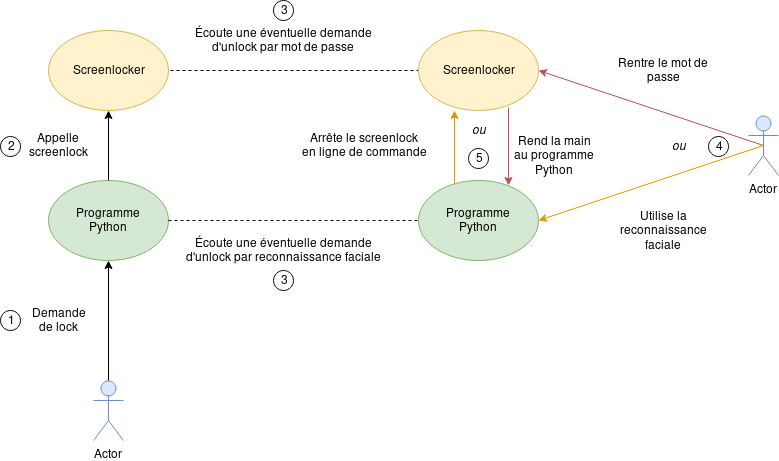
\includegraphics[width=\linewidth]{diagramme_lockatme}
  \caption{diagramme appel programme tier}
\end{figure}
